\chapter{Introduction}
Nonlinear systems\cite{sastry2013nonlinear} \cite{iqbal2017nonlinear}, as their name suggests, do not exhibit linear relationships between inputs and outputs. This means their responses can't be simply predicted using linear equations. In the real world, nearly all systems display some degree of nonlinearity, which can manifest in various phenomena. For instance, in systems with multiple inputs and outputs (MIMO), the relationships between input and output variables can become interdependent, leading to coupling issues. A widely-discussed challenge that arises from nonlinearity is chaotic behavior\cite{ditto1995principles}\cite{oestreicher2007history}, where minor changes in initial conditions can lead to vastly different outcomes. 

Achieving precise control over nonlinear systems has long been a primary focus in the field of control theory. While linear systems, often represented by linear differential equations, can typically be solved quickly and analytically, nonlinear equations representing nonlinear dynamics usually lack closed-form solutions\cite{struble2018nonlinear}. This necessitates the use of approximations and numerical methods. Executing these methods efficiently and accurately presents a central challenge in nonlinear control. Throughout history, control engineers have devised a wide range of strategies to manage a variety of complex systems. The rise of robotics in recent decades has introduced new methods specifically tailored to address the challenges presented by nonlinearities.

\section{Motivation}
Robots are purposefully engineered as programmable mechanical structures, enabling them to perform a variety of tasks, either autonomously or partial under human supervision. Typical tasks include mobility, manipulation, and active interaction with their surroundings.

In the field of modern robotics, the mechanical systems are highly complex and nonlinear, posing significant challenges for precise and effective control. However, with the advancement of modern control methodologies and the increasing capabilities of artificial intelligence, numerous innovative control approaches are emerging each year. Many products in modern robotics have achieved remarkable commercial success, some well-known instances include quadruped robotics\cite{biswal2021development}, autonomous vehicles\cite{schwarting2018planning}, quadcopters\cite{luukkonen2011modelling}, and humanoid robots\cite{saeedvand2019comprehensive}.

\begin{figure}[H]
    \centering
    \begin{subfigure}[b]{0.45\textwidth}
        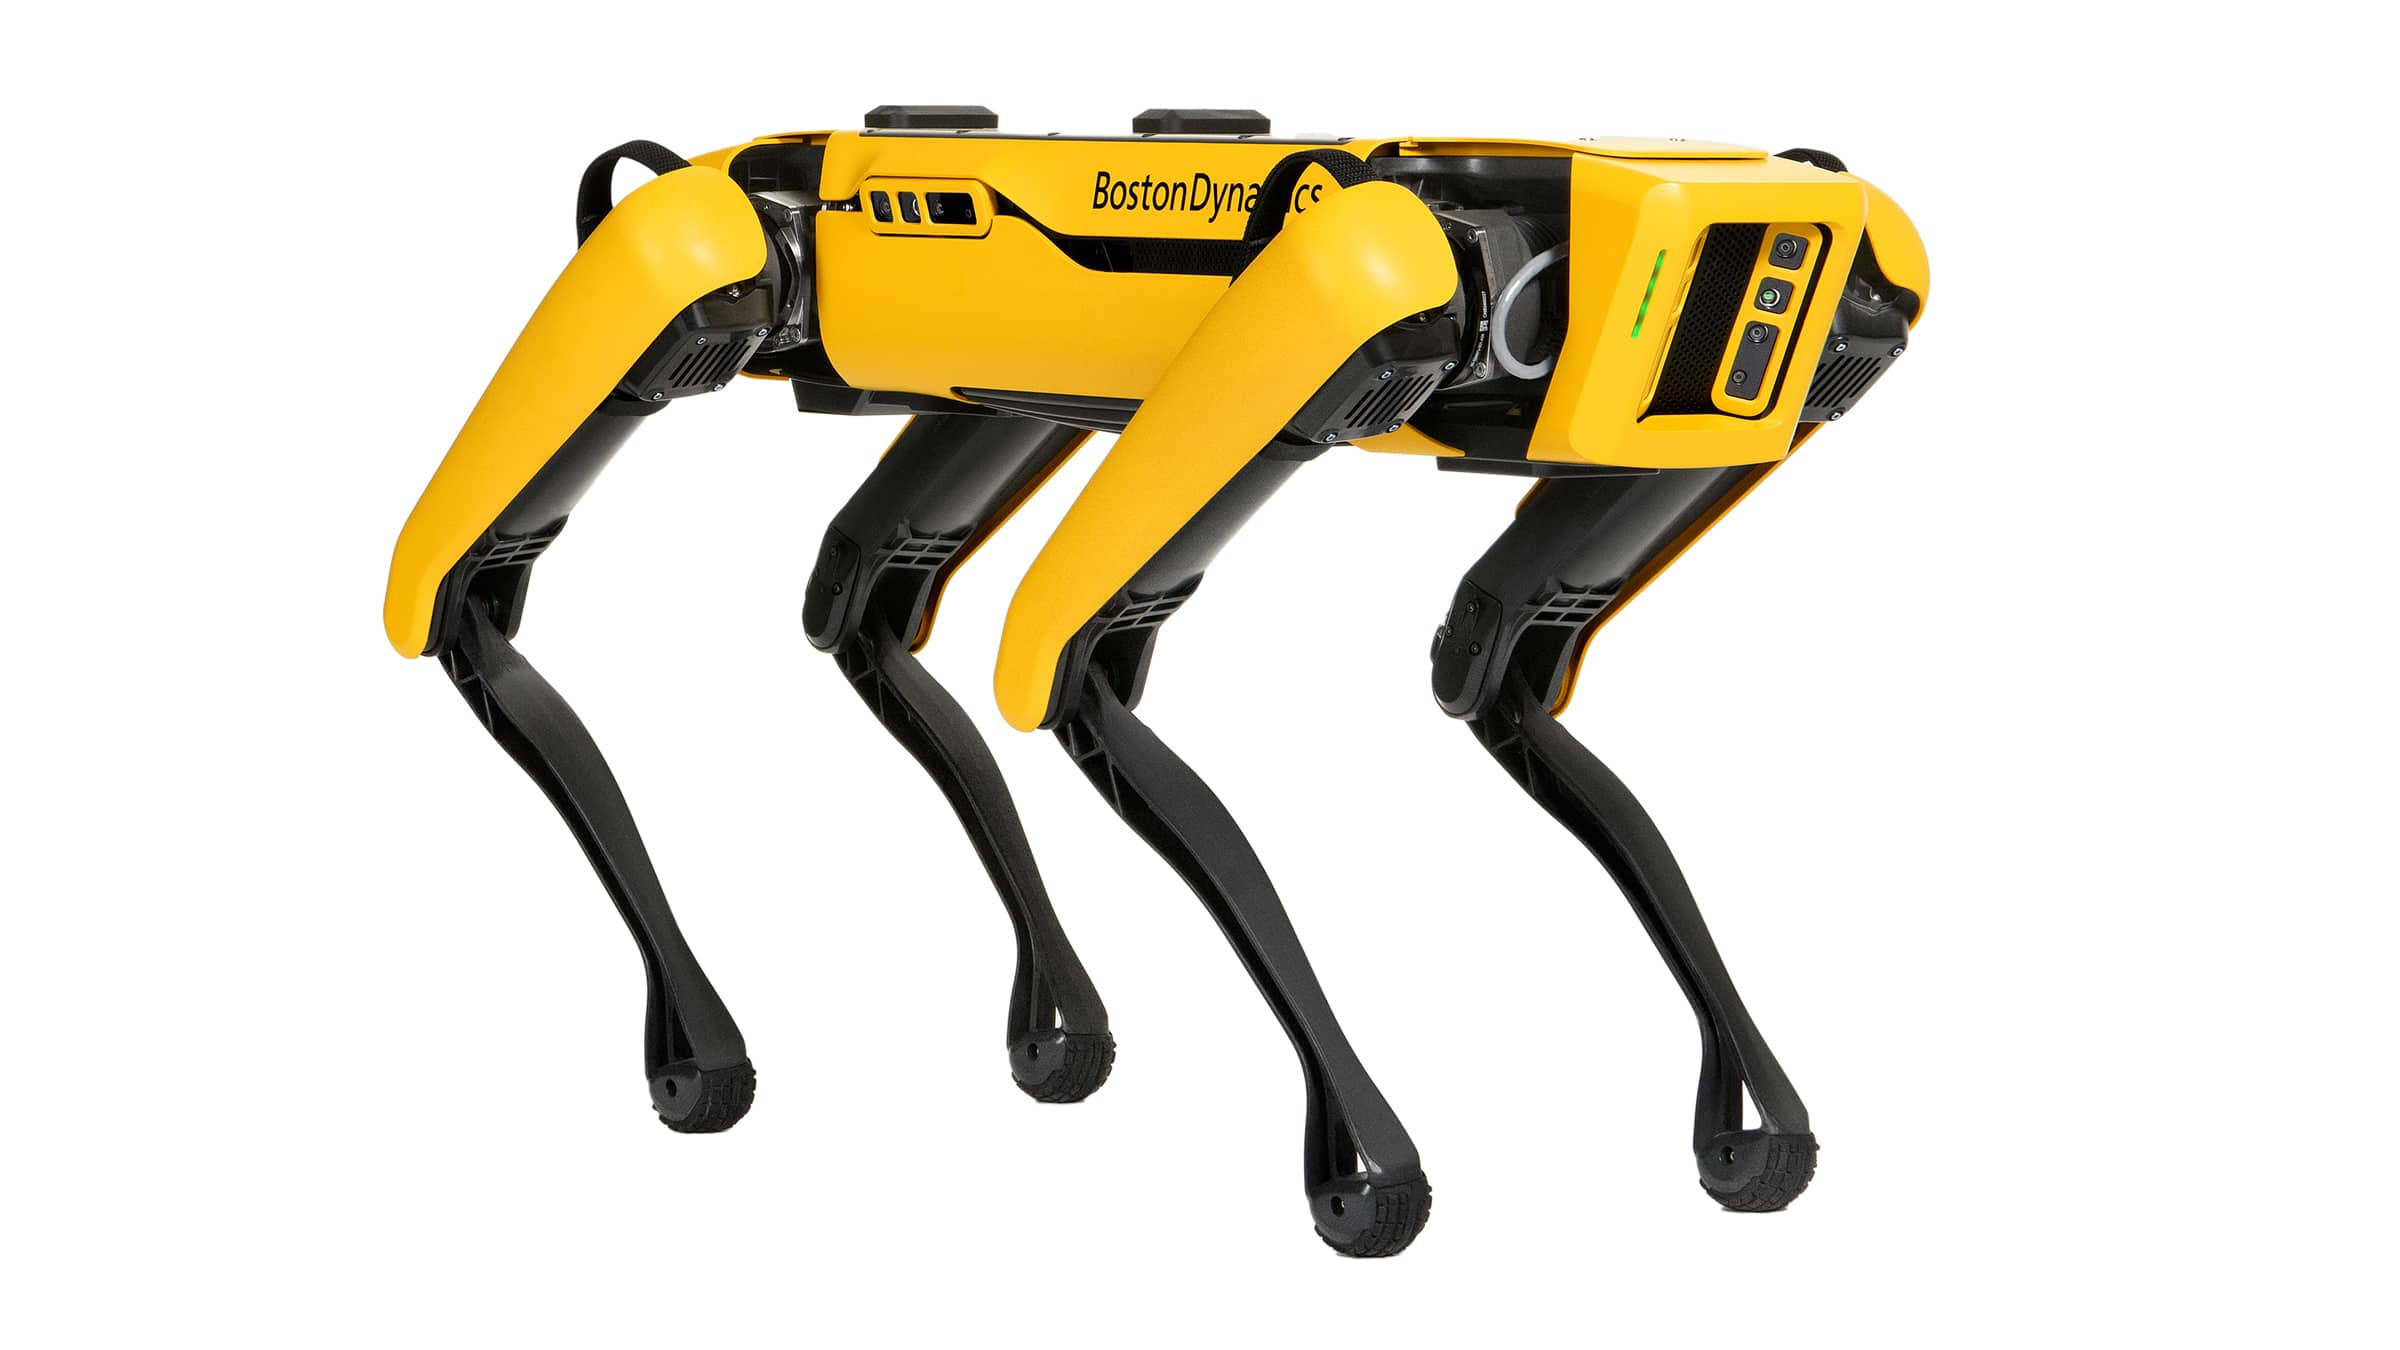
\includegraphics[width=\textwidth]{figures/quadruped.jpg}
        \caption{Quadruped}
        \label{fig:image1}
    \end{subfigure}
    \hfill
    \begin{subfigure}[b]{0.45\textwidth}
        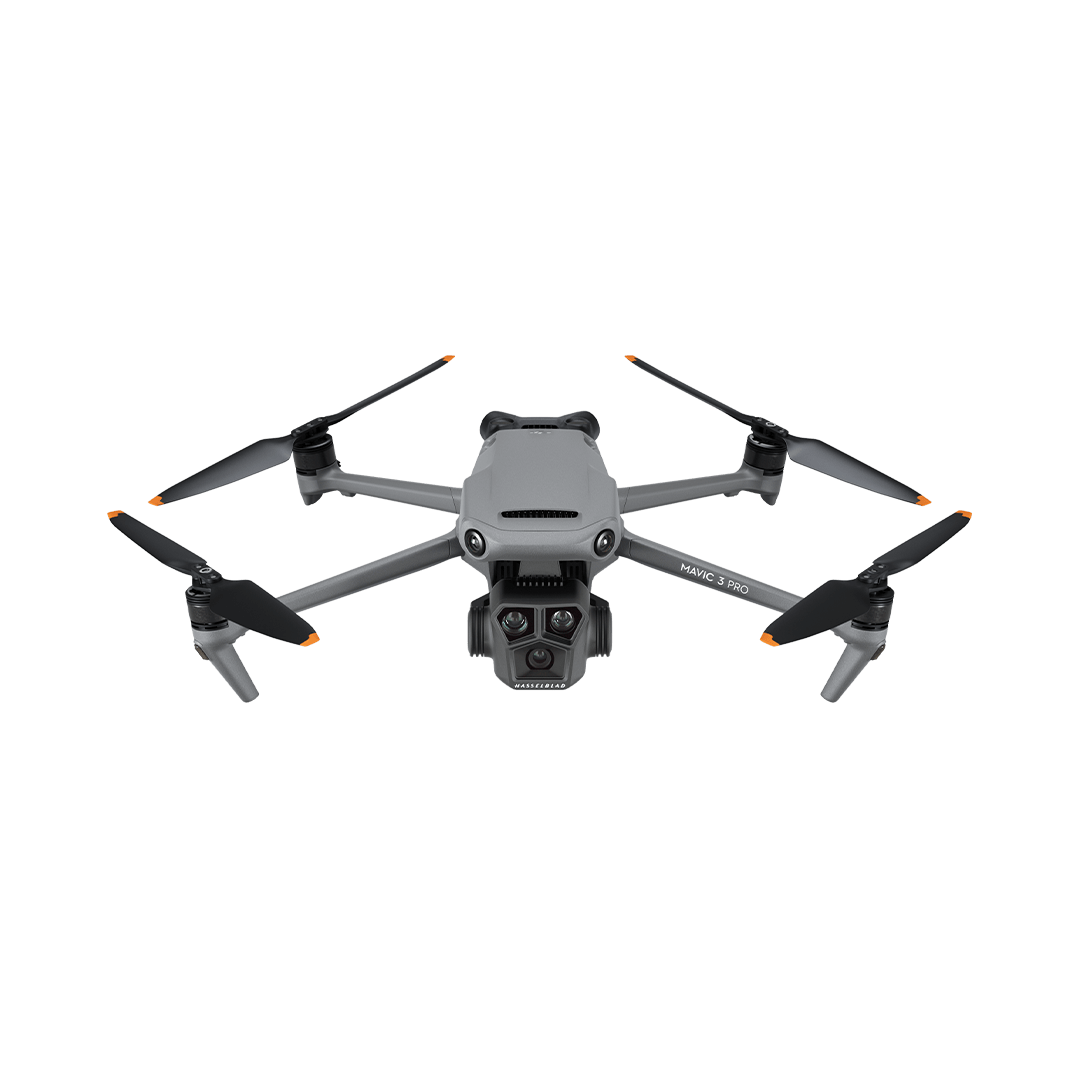
\includegraphics[width=\textwidth]{figures/quadcopter.png}
        \caption{Quadcopter}
        \label{fig:image2}
    \end{subfigure}

    \vspace{1em} % or use \bigskip or \medskip depending on the space you want

    \begin{subfigure}[b]{0.45\textwidth}
        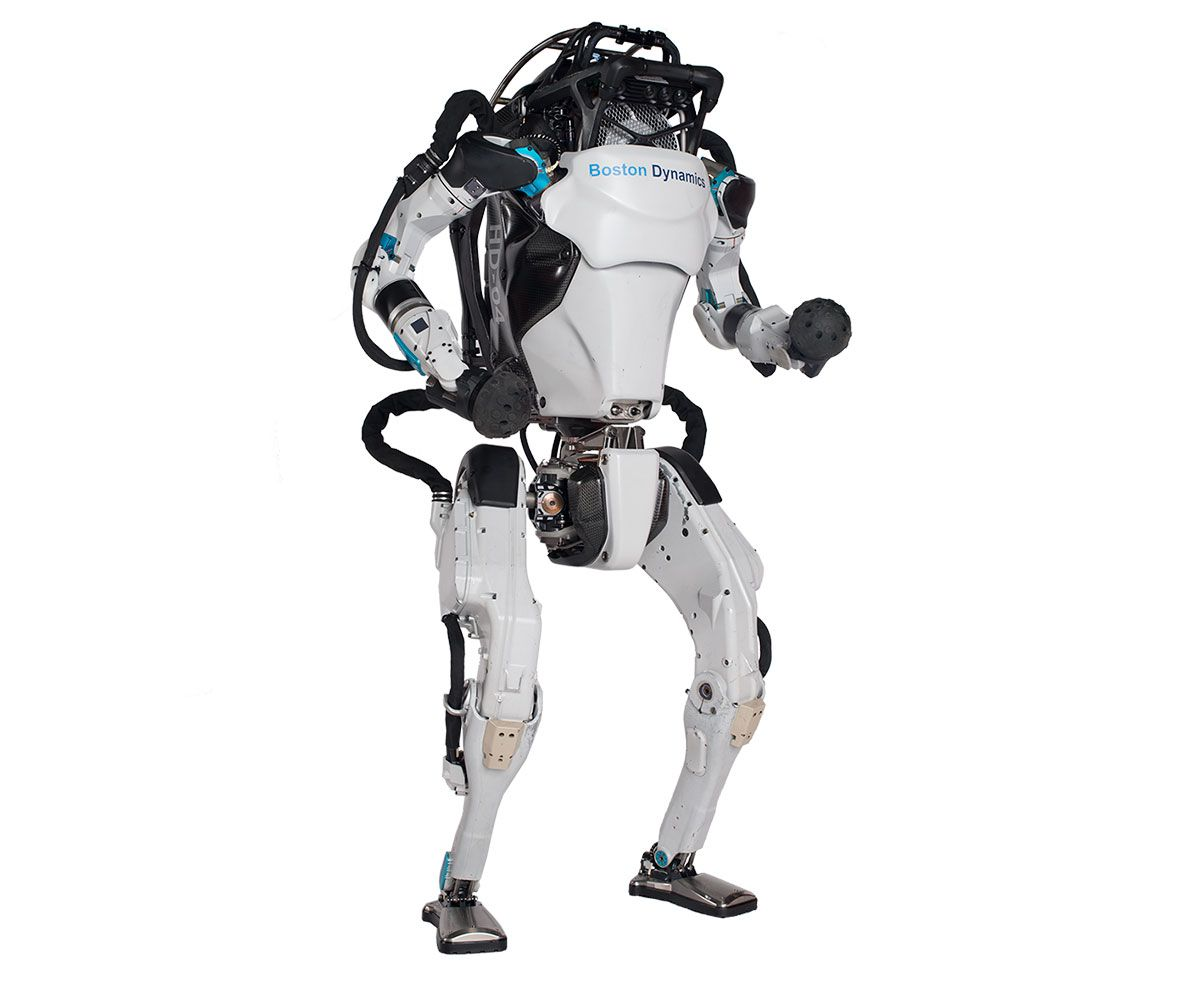
\includegraphics[width=\textwidth]{figures/humanoid.jpg}
        \caption{Humanoid}
        \label{fig:image3}
    \end{subfigure}
    \hfill
    \begin{subfigure}[b]{0.45\textwidth}
        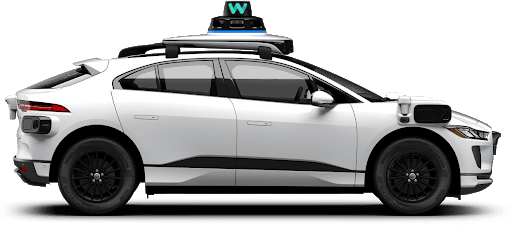
\includegraphics[width=\textwidth]{figures/waymo.png}
        \caption{Autonomous vehicle}
        \label{fig:image4}
    \end{subfigure}
    \caption{Four successful examples for controlling dynamic and nonlinear systems in the field of modern robotics}
    \label{fig:four_images}
\end{figure}

\subsection{Trajectory planning and tracking}
In the traditional control of complex systems such as robotics, which exhibit significant nonlinearity, it is crucial to employ reliable nonlinear control strategies to guarentee motion capabilities. Typically, the procedure for executing precise motion within these systems subjects to a two-phase method\cite{biagiotti2008trajectory}, encompassing trajectory planning and trajectory tracking. This structured approach ensures precision and stability in robotic system control.

Trajectory planning\cite{gasparetto2015path}\cite{gasparetto2012trajectory} involves calculating a smooth and feasible path for the robot to follow, aiming for a specific target position or operational point. A widely-used method in this stage, trajectory optimization\cite{betts1998survey}, seeks to minimize a cost function that accounts for metrics like travel time, energy consumption, and motion smoothness. Techniques such as gradient descent or genetic algorithms are often utilized for optimization. These techniques are subject to constraints, with aspects like maximum velocities and accelerations being crucial in the process.

Upon successful trajectory planning, the next step is trajectory tracking, which requires the use of control algorithms to guide the robot along the predetermined path. A feedback control approach is typically employed, continually monitoring the robot's position and adjusting control inputs as necessary. However, in real-world systems, external disturbances, uncertainties, and system limitations may lead to significant deviations from the planned trajectory. Therefore, ensuring accurate state estimation and implementing robust control strategies are imperative in feedback control to address these challenges.

Below, two examples of trajectory-based control are discussed. In conventional industrial robot control\cite{gasparetto2010optimal}, it is typical for the control process to be divided into distinct phases of offline planning and execution. This segmentation is primarily due to the non-critical need for real-time responsiveness in such applications. Consider the planning phase, for example, where an optimal route is determined by an algorithm such as A*, based on a predefined task. Tasks often include navigating around obstacles and minimizing travel distance, leading to the generation of a set of discrete waypoints\cite{cui2011based}. These waypoints are then subjected to cubic interpolation techniques\cite{bickley1968piecewise}, resulting in the crafting of a smooth and continuous trajectory that can be realistically followed by the robot. This approach ensures not only seamless motion but also compliance with the robot's kinematic constraints. Subsequently, the process transitions to the execution phase, during which a robust and precise control strategy, such as PID, is implemented. This strategy is crucial, as it ensures the robot's adherence to the pre-established trajectory, maintaining accuracy and reliability throughout the operation\cite{lynch2017modern}.

Yet, in dynamic domains like automotive and flight control, the demand for real-time responsiveness takes center stage. In such cases, Model Predictive Control (MPC)\cite{kouvaritakis2016model} serves as a key example of integrating online trajectory planning and execution, meeting the critical need for real-time responsiveness. In the planning phase, MPC forecasts a series of future control actions. This is achieved by minimizing discrepancies between the current observed state and the intended trajectory. Once the planning is complete, MPC implements the first set of these predicted control inputs during the execution phase. Immediately following this implementation, the system's new state is observed and fed back into the MPC algorithm. This leads to a re-evaluation and update of the future control actions in what becomes a continuous, iterative process. MPC's strength lies in its ability to simultaneously create, optimize, and follow trajectories, dynamically adjusting in real-time to address any disturbances and uncertainties. Such capability is essential for ensuring precise control and adaptability in complex systems that operate in real-time environments.

In conclusion, the traditional trajectory planning and tracking approach, while effective for numerous systems, has its own set of limitations.

\begin{itemize}
    \item \textbf{Limited Adaptability:} 
    Trajectory planning typically relies on predefined paths or trajectories, limiting adaptability to unforeseeable changes or dynamic environments. If the environment changes significantly during execution, the planned trajectory may no longer be optimal or even feasible.
        
    \item \textbf{Difficulty with Nonlinear Systems:} 
    Trajectory planning struggles with highly nonlinear systems where the dynamics are hard to model accurately. Linearizing the system for planning purposes may lead to suboptimal or infeasible trajectories.
    
    \item \textbf{High Computational Demands:} 
    Some trajectory planning algorithms can be computationally intensive, especially for high-dimensional or complex robotic systems. This computational demand becomes a drawback, particularly in real-time or time-critical applications.
\end{itemize}

% Recognizing the limitations inherent in traditional trajectory planning and tracking methodologies is essential for fostering the development of more advanced and efficient strategies in trajectory planning and control. This insight becomes particularly crucial in contexts that require rapid responsiveness and a capacity to skillfully navigate unpredictable changes or dynamic environments.

\subsection{Reinforcement Learning Based Control}
Transitioning from a focus on predefined trajectories, reinforcement learning(RL)-based control presents an alternative framework.

Reinforcement learning (RL)\cite{sutton2018reinforcement} is a subset of machine learning that focuses on agents learning optimal behavior through trial-and-error interactions with their environments. Essentially, the trained agent makes sequential decisions, observes the outcomes of its actions, and receives feedback in the form of rewards or penalties. This feedback serves as a guiding mechanism, enabling the agent to evaluate the outcomes of its actions. It then adjusts its policy accordingly to maximize cumulative rewards over time.

The mathematical framework that describes RL is the Markov Decision Process (MDP)\cite{puterman1990markov}, which provides a structured model for the decision-making problem. In an MDP, the agent's current state, the available actions, the potential next states, and the rewards associated with state-action transitions are all clearly defined. MDPs require the fulfillment of the Markov property, which states that the future state of the system depends only on the current state and the action taken.

\begin{figure}[h]
    \centering
    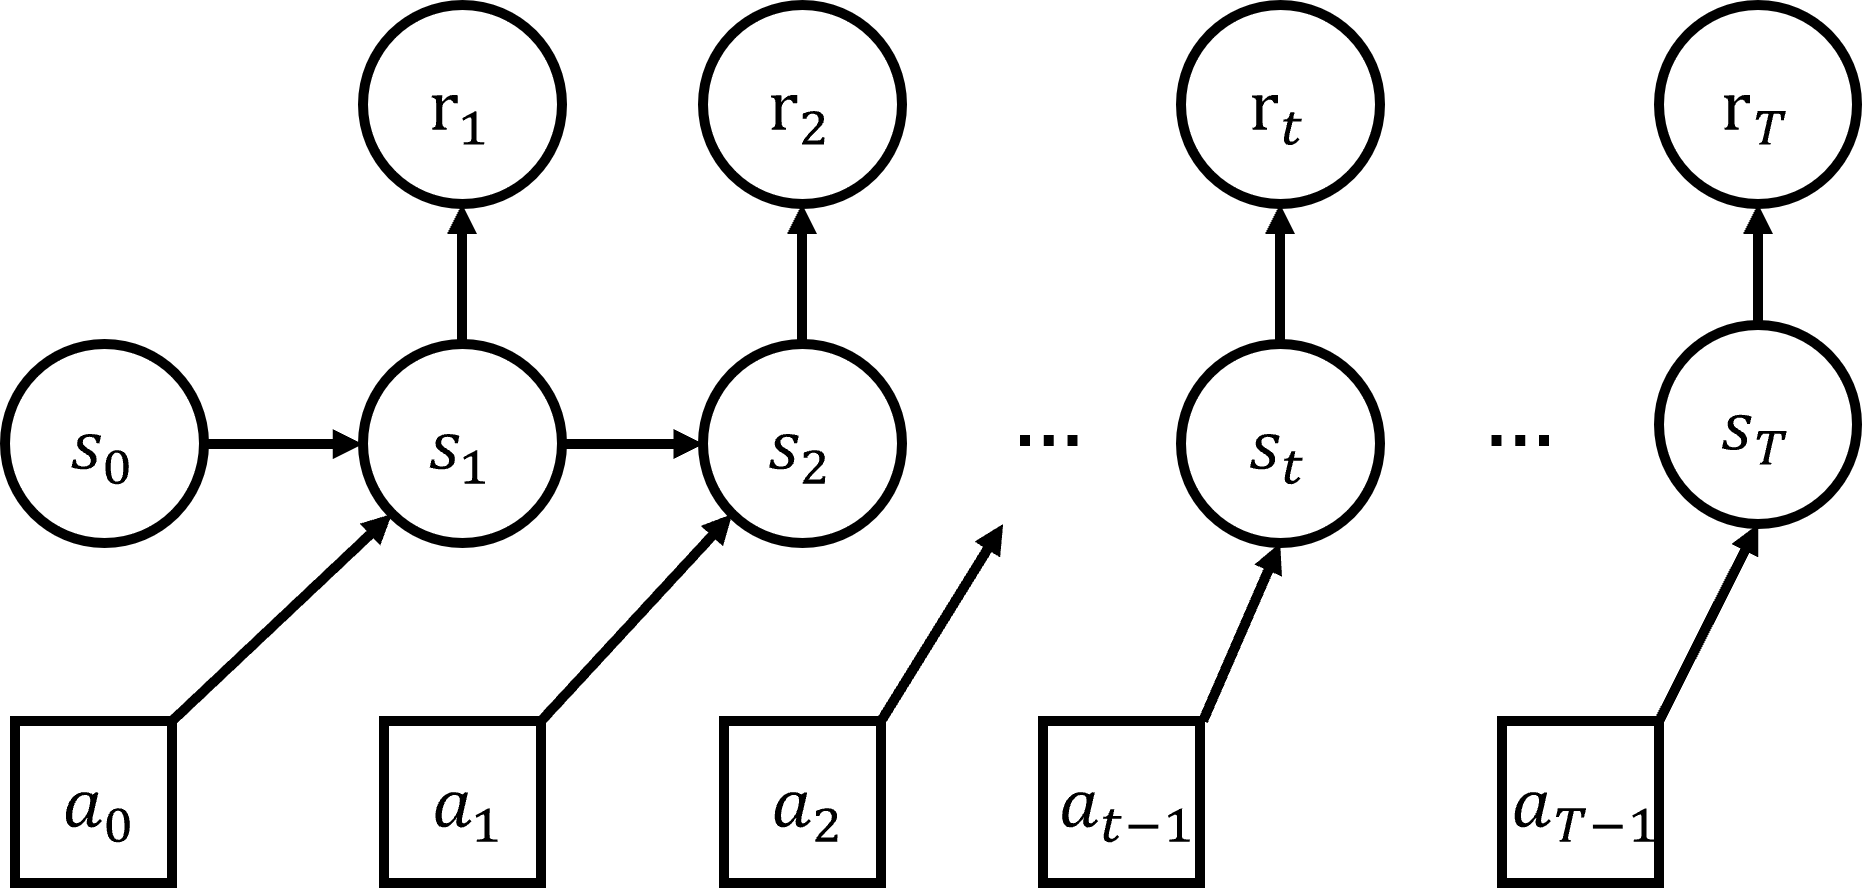
\includegraphics[width=0.8\textwidth]{figures/MDP.png}
    \caption{Markov decision process}
    \label{fig:mdp}
\end{figure}

The ultimate objective in reinforcement learning (RL) is to discover an optimal policy. This policy is a strategic mapping from states to actions, designed to select the most beneficial action in each state to achieve maximum long-term rewards. The learning process is dependent on the tuple \((s, a, r, s')\), which describes the current state \(s\), the action taken \(a\), the reward received \(r\), and the subsequent state \(s'\). Over time, the agent engages in exploring the state and action space to gather information about the effects of various actions, which is essential for acquiring new knowledge. This exploration is complemented by exploitation, where the agent utilizes its accumulated 
knowledge to make informed decisions.

Maintaining a balance between exploration and exploitation is a key challenge in RL. It is crucial for the agent to effectively navigate its environment and learn from the rewards it receives. Through this iterative process of exploration and exploitation, the agent continuously refines and updates its policy. Gradually, this leads to the convergence towards optimal behavior, where the policy consistently yields the highest possible rewards within the constraints of the environment.

In the field of robotics, the integration of reinforcement learning in control tasks\cite{kober2013reinforcement} has become increasingly popular due to the numerous distinct advantages this approach offers:

\begin{itemize}
    \item \textbf{Adaptability and Flexibility:}
    RL allows systems to adapt and improve in dynamic environments; its control policy evolves through accumulating new experiences and knowledge from interactions with the environment, making it highly adaptable to varying circumstances.

    \item \textbf{Reduced Dependency on Accurate Models:}
    In contrast to traditional control methods that depend on exact mathematical models, RL works without the necessity of a predetermined model, particularly when learning from real-world data. This feature is immensely beneficial in situations where the system dynamics are either complex or not well understood, as RL refines its performance through direct interactions with the environment.

    \item \textbf{Effective Handling of Nonlinearities and High-Dimensional Systems:}
    RL excels at managing nonlinear systems and complex control tasks using neural network-based function approximation. This enables it to navigate high-dimensional input and output spaces and deal with coupling problems in multiple input and output systems.
\end{itemize}

In conclusion, reinforcement learning is a straightforward control method with high adaptability, setting itself apart from traditional trajectory planning and tracking techniques. While conventional methods frequently struggle with challenges such as limited adaptability, nonlinearity in systems, and intensive computational demands, reinforcement learning addresses these issues through direct interactions with the environment. It excels in unpredictable conditions and in managing complex, high-dimensional systems. This is largely attributed to its reduced dependency on accurate dynamic models, ensuring robustness, effectiveness, and versatility across a wide range of applications.


\section{Problem setup}
In the realm of nonlinear systems, underactuated systems\cite{liu2013survey} present a particularly challenging class. These systems are characterized by having fewer control inputs than degrees of freedom, or their control inputs are constrained in some way. This characteristic makes them significantly more challenging to control when compared to fully actuated systems. What's intriguing is that a majority of robots and even natural organisms fall into the category of underactuated systems. Consequently, the study of underactuated mechanical systems' control holds universal relevance.

The concept of underactuated dynamics can be briefly introduced as follows. According to Newton's second law (\( F = ma \)), the dynamics that govern any mechanical system can be mathematically expressed as shown in Equation \ref{eq:nonlinear_dynamics_general_form}:

\begin{align}
    \ddot{q} = f(q, \dot{q}, u, t)
    \label{eq:nonlinear_dynamics_general_form}
\end{align}

In this equation, \( \ddot{q} \) represents acceleration, which is the second derivative of the variable \( q \), typically representing the position of the system. The function \( f(q, \dot{q}, u, t) \) describes how \( \ddot{q} \) depends on various parameters, including the state variables \( q \) and \( \dot{q} \), the control inputs \( u \), and the time \( t \).

The state of the system, denoted as \( x \) and represented as \( [q, \dot{q}]^T \), consists of two vectors: \( q \), which signifies positions, and \( \dot{q} \), which signifies velocities.

When dealing with control-affine systems, we can express the second-order differential equation in the following manner:

\begin{align}
    \ddot{q} = f_1(q, \dot{q}, t) + f_2(q, \dot{q}, t)u
    \label{eq:nonlinear_dynamics_control_form}
\end{align}

In this equation, \( f_1(q, \dot{q}, t) \) corresponds to one part of the function that affects \( \ddot{q} \), while \( f_2(q, \dot{q}, t) \) represents another part that interacts with the control input \( u \).

In the context of a controlled dynamical system, as described by Equation \ref{eq:nonlinear_dynamics_control_form}, we evaluate the condition of underactuation at specific states \([q, \dot{q}]^T\) at time \(t\). Underactuation can be identified through two distinct scenarios:

\begin{itemize}
 \item \textbf{Case 1:}
 
 The system is classified as underactuated at a particular state if the rank of the matrix \([f_2(q, \dot{q}, t)]\) is less than the dimension of \(q\). This condition is expressed as:
 
 \begin{align}
    \text{rank}[f_2(q, \dot{q}, t)] < \text{dim}[q]
\end{align}
 
 \item \textbf{Case 2:} 
 
 Alternatively, underactuation may also arise even when \(f_2\) is full rank, provided there are additional constraints on the control inputs. For instance, if constraints such as \(|\mathbf{u}| \leq 1\) limit the control inputs, the system's controllability can still be restricted, resulting in underactuation.
\end{itemize}

These principles are explained in the work by Russ Tedrake\cite{tedrake2022underactuated}.

A well-discussed example of underactuated control is found in the double pendulum—a simple setup consisting of two links connected by two rotational joints. These joints include the shoulder joint, which is directly connected to the world frame, and the elbow joint, situated between the two links. The end effector is located at the tip of the second link. Active control is achieved by attaching motors to the shoulder and elbow joints. In the domain of underactuated control, if the shoulder joint is actuated, the setup is referred to as a pendubot (see Figure \ref{pendubot_explained}). Conversely, if the elbow joint is actuated, it is known as an acrobot (see Figure \ref{acrobot_explained}).

\begin{figure}[htbp]
    \centering
    \begin{subfigure}[b]{0.2\textwidth}
        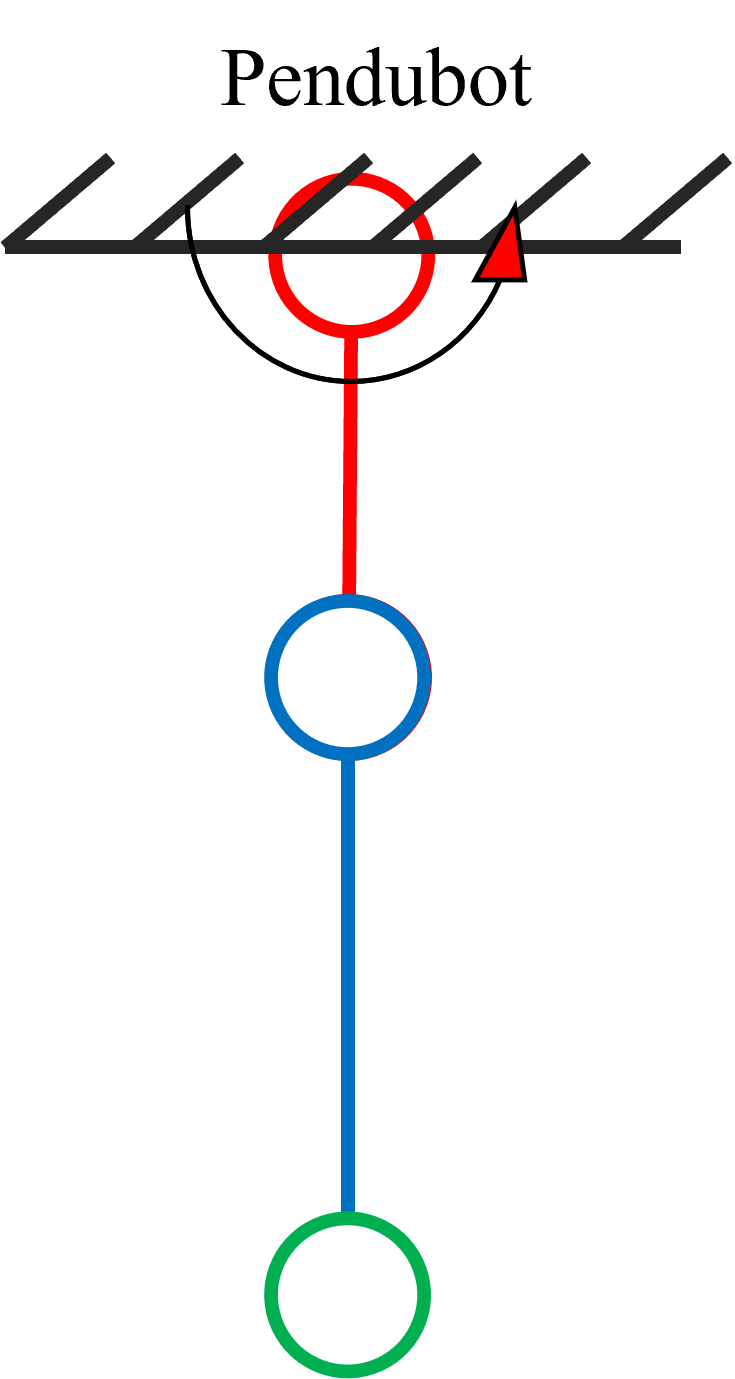
\includegraphics[width=\textwidth]{figures/pendubot_explained.png}
        \caption{Pendubot setup}
        \label{pendubot_explained}
    \end{subfigure}
%     \hfill
    \begin{subfigure}[b]{0.2\textwidth}
        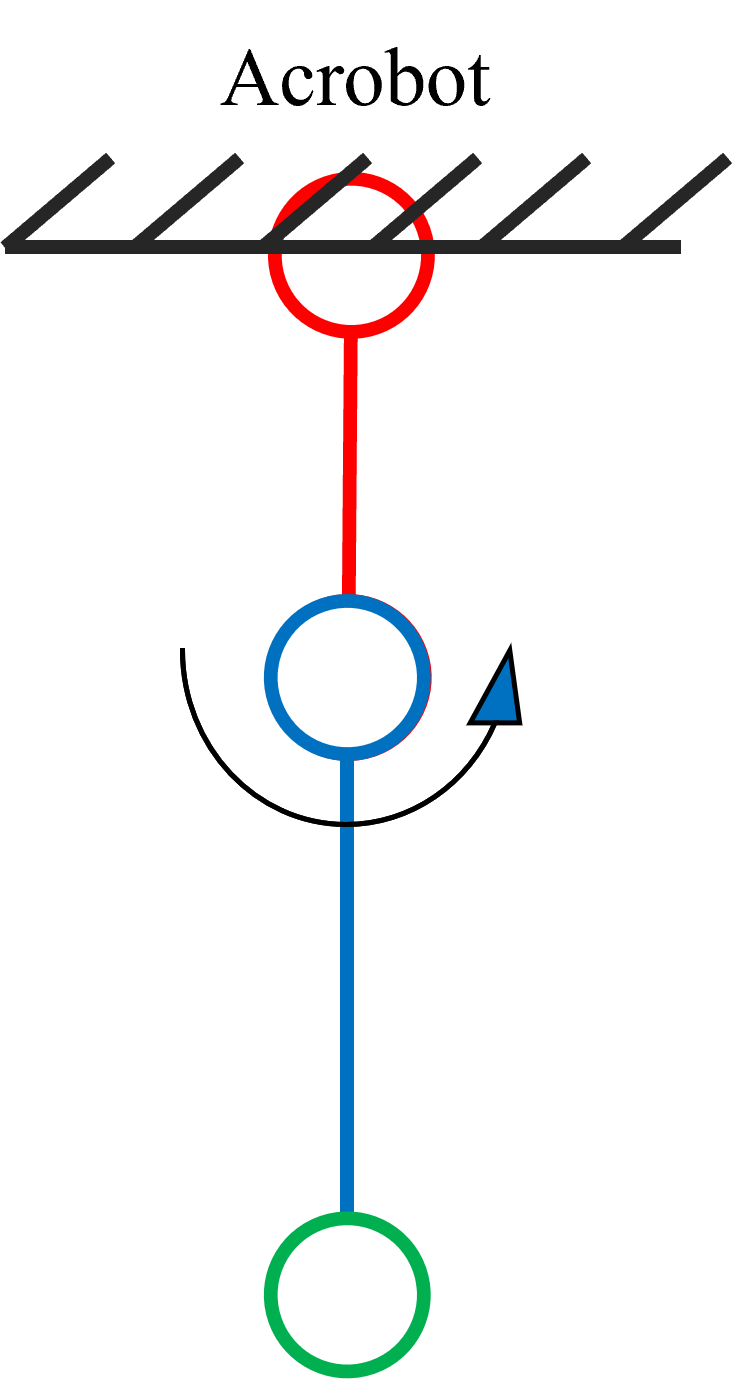
\includegraphics[width=\textwidth]{figures/Acrobot_explained.png}
        \caption{Acrobot setup}
        \label{acrobot_explained}
    \end{subfigure}
    \caption{Two variations of underactuated double pendulum}
\end{figure}

Despite its simple configuration, the system exhibits highly nonlinear and chaotic behavior\cite{shinbrot1992chaos}. The double pendulum setup presents two classic tasks: swing-up and stabilization around the highest point. Research on swing-up and stabilization of the double pendulum can be traced back to the 1990s\cite{yamakita1995robust}, and it continues to be a crucial testbed for validating the effectiveness of newly designed control algorithms\cite{xin2004new}\cite{zheng2006control}\cite{albahkali2009swing}.

Our project's objective is to develop a reinforcement learning-based control method suitable for underactuated control of the double pendulum system, specifically addressing swing-up and stabilization tasks. To evaluate the efficacy of this control method, we conduct both simulations and real system experiments. The real system setup is shown in Figure \ref{fig:double_pendulum_real_system}

\begin{figure}[H]
    \centering
    \includegraphics[width=0.45\textwidth]{figures/double_pendulum_real_system.png}
    \caption{Double pendulum in real system}
    \label{fig:double_pendulum_real_system}
\end{figure}

\section{Contribution}
In this thesis, the primary contribution is the development of an effective control strategy for a double pendulum to achieve two key objectives. The first objective involves swinging the double pendulum from its lowest point to its highest point. The second objective is to ensure stability at the highest point over an extended period.

For the swing-up task, a well-known model-free reinforcement learning algorithm, Soft Actor-Critic (SAC), was employed\cite{haarnoja2018soft}. This algorithm enabled the training of a policy capable of reaching the Region of Attraction (RoA) of a continuous-time linear quadratic regulator (LQR) controller\cite{lehtomaki1981robustness}. Upon reaching the RoA, the system transitions seamlessly to the LQR controller, maintaining stability around the highest point.

The findings from the simulation and real hardware tests were presented at the IJCAI 2023 conference in Macau, in the RealAIGym competition\cite{dfki_ric_underactuated_lab_2023}. Furthermore, this work has been made available as open source, accessible at:

\url{https://github.com/dfki-ric-underactuated-lab/double_pendulum}.

\section{Content}
This thesis comprises seven chapters, namely: Introduction, State of the Art, Methodology, Agent Training and Experiments in a Simulation Environment, Experiments on Real Hardware, Discussion, and Conclusion and Future Work. At the end of Chapter 1, the content of the following chapters is outlined below.

\begin{itemize}
  \item \textbf{Chapter 2: State of the Art}:
    \begin{itemize}
      \item In this chapter, an explanation is provided on the fundamental theories related to double pendulum dynamics, followed by an overview of recent advancements in the field of robotic control, with a particular emphasis on learning-based control methods.
    \end{itemize}
  
  \item \textbf{Chapter 3: Methodology}:
    \begin{itemize}
      \item The methodology is explored in this chapter, covering fundamental aspects of reinforcement learning, with a specific focus on the SAC algorithm. The reward function used for training, the training procedure, and the concept of the LQR controller and the composition of the combined controller are explained. Furthermore, evaluation metrics used to assess the performance and robustness of the newly designed control strategies in both simulated environments and real-world experiments are introduced.
    \end{itemize}

  \item \textbf{Chapter 4: Agent Training and Experiments in Ideal Simulation Environments}:
    \begin{itemize}
      \item The training process of agents based on the SAC algorithm in ideal simulation environments is presented in this chapter. Additionally, results obtained from these simulations are demonstrated to showcase the performance and behavior of the designed control strategy.
    \end{itemize}
  
  \item \textbf{Chapter 5: Experiments on Real Hardware}:
    \begin{itemize}
      \item The hardware setup, including mechanics, electronics, and safety measures, is explained first in this chapter. Subsequently, system identification is introduced. The approach for bridging the sim-to-real gap is discussed next, encompassing the setting up of noisy simulations for evaluation and a noisy training process based on domain randomization. The process for selecting the suitable agent for real-world tests is also introduced. Finally, the outcomes of experiments conducted on the real hardware are provided, highlighting that the combined controller is functional only on the pendubot.
    \end{itemize}
  
  \item \textbf{Chapter 6: Discussion}:
    \begin{itemize}
      \item A discussion on the obtained results is undertaken in this chapter, including a comparison of the performance and robustness leaderboards in simulations and the performance leaderboards in the real world.
    \end{itemize}
  
  \item \textbf{Chapter 7: Conclusion and Future Work}:
    \begin{itemize}
      \item The final chapter offers a conclusion of the work and the results obtained. It also discusses future work that was not completed in this thesis.
    \end{itemize}
\end{itemize}






\cleardoublepage
